\documentclass{article}
\usepackage{tikz}
\usetikzlibrary{shapes}
\usetikzlibrary{calc}
\usepackage{amsmath}
\usepackage{amssymb}
\begin{document}

\section{Procrastination MDP}
\label{sec:procrastination-mdp}
\vspace{1cm}
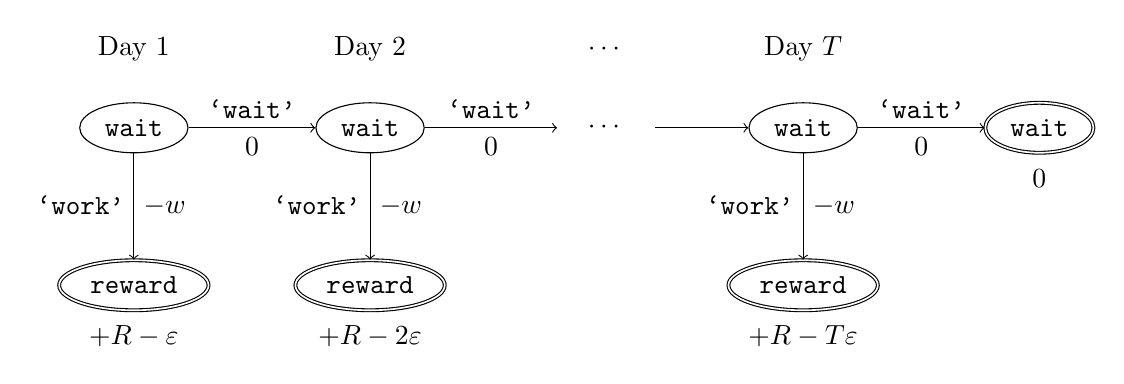
\begin{tikzpicture}
  \node (day1) at (0,3) {Day 1};
  \node (day2) at (3,3) {Day 2};
  \node (daysellipsis) at (6,3) {$\dotsb$};
  \node (dayt) at (8.5,3) {Day $T$};
  
  \node[draw, ellipse] (wait1) at (0,2) {\texttt{wait}};
  \node[draw, ellipse] (wait2) at (3,2) {\texttt{wait}};
  \node (waitellipsis-) at (5.5,2) {};
  \node (waitellipsis) at (6,2) {$\dotsb$};
  \node (waitellipsis+) at (6.5,2) {};
  \node[draw, ellipse] (wait3) at (8.5,2) {\texttt{wait}};
  \node[draw, double, ellipse] (wait4) at (11.5, 2) {\texttt{wait}};
  \node (utilityAtDeath) at (11.5, 1.35) {$0$};
  
  \node[draw, double, ellipse] (reward1) at (0,0) {\texttt{reward}};
  \node[draw, double, ellipse] (reward2) at (3,0) {\texttt{reward}};
  \node[draw, double, ellipse] (reward3) at (8.5,0) {\texttt{reward}};
  \node (utilityReward1) at (0, -0.65) {$+R - \varepsilon$};
  \node (utilityReward1) at (3, -0.65) {$+R - 2 \varepsilon$};
  \node (utilityReward1) at (8.5, -0.65) {$+R - T \varepsilon$};

  \draw[->] (wait1) -- node[above] {\texttt{`wait'}} node[ below] {$0$} (wait2);
  \draw[->] (wait2) -- node[above] {\texttt{`wait'}} node[ below] {$0$} (waitellipsis-);
  \draw[->] (waitellipsis+) -- (wait3);
  \draw[->] (wait3) -- node[above] {\texttt{`wait'}} node[ below] {$0$} (wait4);

  \draw[->] (wait1) -- node[left] {\texttt{`work'}} node[right] {$-w$} (reward1);
  \draw[->] (wait2) -- node[left] {\texttt{`work'}} node[right] {$-w$} (reward2);
  \draw[->] (wait3) -- node[left] {\texttt{`work'}} node[right] {$-w$} (reward3);

\end{tikzpicture}
\vspace{1cm}
\section{POMDP model}
\label{sec:pomdp-model}

\vspace{1cm}
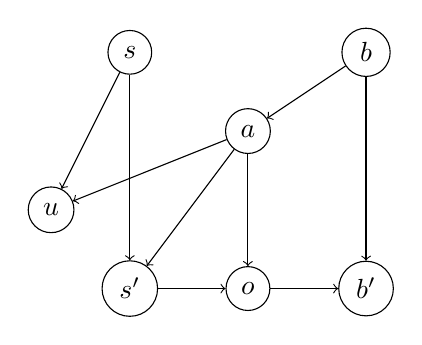
\begin{tikzpicture}
  \node[draw, circle] (st) at (1,3) {$s$};
  \node[draw, circle] (bt) at (4,3) {$b$};
  \node[draw, circle] (at) at (2.5,2) {$a$};
  \node[draw, circle] (ut) at (0,1) {$u$};
  \node[draw, circle] (st+1) at (1,0) {$s'$};
  \node[draw, circle] (ot+1) at (2.5,0) {$o$};
  \node[draw, circle] (bt+1) at (4,0) {$b'$};

  \path[->] (st) edge (st+1);
  \path[->] (bt) edge (at);
  \path[->] (at) edge (ut);
  \path[->] (st) edge (ut);
  \path[->] (at) edge (st+1);
  \path[->] (st+1) edge (ot+1);
  \path[->] (at) edge (ot+1);
  \path[->] (ot+1) edge (bt+1);
  \path[->] (bt) edge (bt+1);
\end{tikzpicture}
\vspace{1cm}

\section{IRL Bandits}
\label{sec:irl-bandits}

\subsection{3c, first todo}
\label{sec:3c-first-todo}


\vspace{1cm}

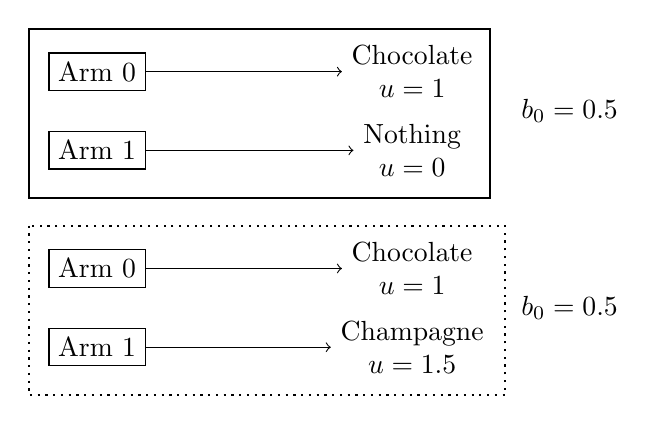
\begin{tikzpicture}
  \node[draw, rectangle] (arm0) at (0,1) {Arm 0};
  \node[draw, rectangle] (arm1) at (0,0) {Arm 1};
  \node[align=center] (prize1) at (4,0) {Champagne \\ $u = 1.5$};
  \node[align=center] (prize0) at (4,1) {Chocolate \\ $u = 1$};

  \path[->] (arm0) edge (prize0);
  \path[->] (arm1) edge (prize1);

  \node[draw, rectangle] (arm0') at (0,3.5) {Arm 0};
  \node[draw, rectangle] (arm1') at (0,2.5) {Arm 1};
  \node[align=center] (prize1') at (4,2.5) {Nothing \\ $u = 0$};
  \node[align=center] (prize0') at (4,3.5) {Chocolate \\ $u = 1$};

  \path[->] (arm0') edge (prize0');
  \path[->] (arm1') edge (prize1');

  \draw[thick] ($(arm0'.north west)+(-0.25,0.3)$) rectangle ($(prize1'.south east)+(0.25,-0.15)$);

  \draw[thick, dotted] ($(arm0.north west)+(-0.25,0.3)$) rectangle ($(prize1.south east)+(0.15,-0.15)$);

  \node (probChamp) at (6, 0.5) {$b_0 = 0.5$};
  \node (probChoc) at (6, 3) {$b_0 = 0.5$};
\end{tikzpicture}

\vspace{1cm}

\subsection{5c}
\label{sec:5c}

\vspace{1cm}

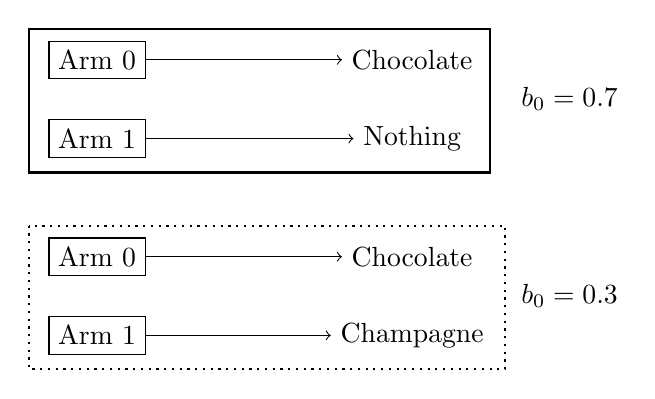
\begin{tikzpicture}
  \node[draw, rectangle] (arm0) at (0,1) {Arm 0};
  \node[draw, rectangle] (arm1) at (0,0) {Arm 1};
  \node[align=center] (prize1) at (4,0) {Champagne};
  \node[align=center] (prize0) at (4,1) {Chocolate};

  \path[->] (arm0) edge (prize0);
  \path[->] (arm1) edge (prize1);

  \node[draw, rectangle] (arm0') at (0,3.5) {Arm 0};
  \node[draw, rectangle] (arm1') at (0,2.5) {Arm 1};
  \node[align=center] (prize1') at (4,2.5) {Nothing};
  \node[align=center] (prize0') at (4,3.5) {Chocolate};

  \path[->] (arm0') edge (prize0');
  \path[->] (arm1') edge (prize1');

  \draw[thick] ($(arm0'.north west)+(-0.25,0.15)$) rectangle ($(prize1'.south east)+(0.25,-0.15)$);

  \draw[thick, dotted] ($(arm0.north west)+(-0.25,0.15)$) rectangle ($(prize1.south east)+(0.15,-0.15)$);

  \node (probChamp) at (6, 0.5) {$b_0 = 0.3$};
  \node (probChoc) at (6, 3) {$b_0 = 0.7$};
\end{tikzpicture}


\vspace{1cm}

\section{Stochastic bandits}
\label{sec:stochastic-bandits}

\subsection{3c}
\label{sec:3c}

\vspace{1cm}

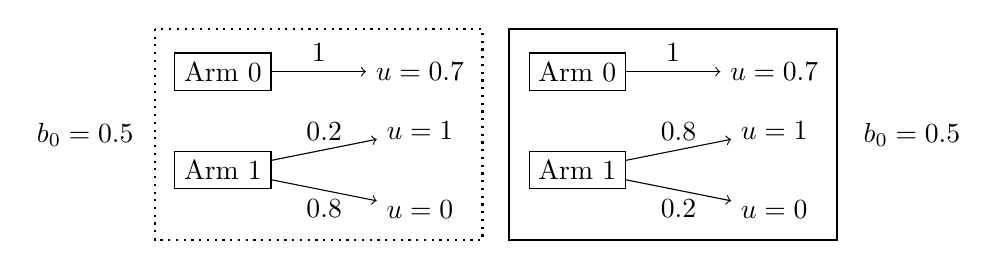
\begin{tikzpicture}
  \node[draw, rectangle] (arm01bad) at (1,1) {Arm 0};
  \node (u01bad) at (3.5,1) {$u = 0.7$};

  \path[->] (arm01bad) edge node[above] {1} (u01bad);

  \node[draw, rectangle] (arm01good) at (5.5,1) {Arm 0};
  \node (u01good) at (8,1) {$u = 0.7$};

  \path[->] (arm01good) edge node[above] {1} (u01good);

  \node[draw, rectangle] (arm1bad) at (1,-0.25) {Arm 1};
  \node (u11bad) at (3.5,0.25) {$u = 1$};
  \node (u10bad) at (3.5,-0.75) {$u = 0$};

  \path[->] (arm1bad) edge node[above] {0.2} (u11bad);
  \path[->] (arm1bad) edge node[below] {0.8} (u10bad);

  \draw[thick, dotted] ($(arm01bad.north west)+(-0.25,0.3)$) rectangle ($(u10bad.south east)+(0.25,-0.15)$);

  \node (probarm1bad) at (-0.75,0.2) {$b_0 = 0.5$};

  \node[draw, rectangle] (arm1good) at (5.5,-0.25) {Arm 1};
  \node (u11good) at (8,0.25) {$u = 1$};
  \node (u10good) at (8,-0.75) {$u = 0$};

  \path[->] (arm1good) edge node[above] {0.8} (u11good);
  \path[->] (arm1good) edge node[below] {0.2} (u10good);

  \draw[thick] ($(arm01good.north west)+(-0.25,0.3)$) rectangle ($(u10good.south east)+(0.25,-0.15)$);

  \node (probarm1good) at (9.75,0.2) {$b_0 = 0.5$};
\end{tikzpicture}


\vspace{1cm}

\subsection{5b myopic}
\label{sec:5b-myopic}


\vspace{1cm}

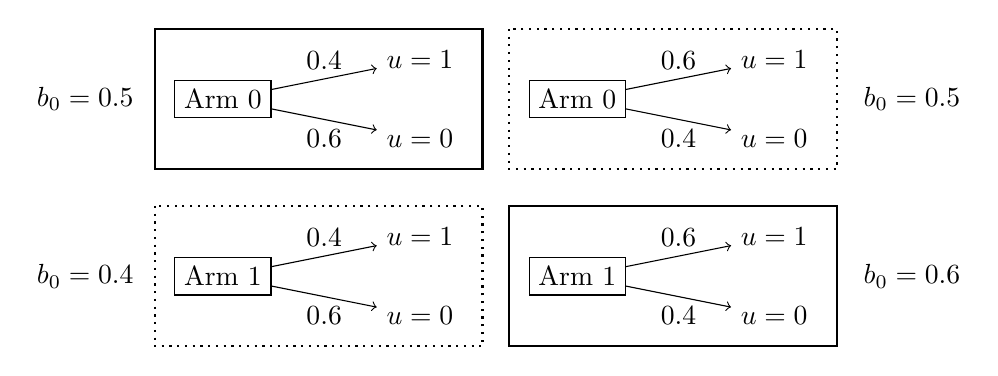
\begin{tikzpicture}
  \node[draw, rectangle] (arm0bad) at (1,2) {Arm 0};
  \node (u01bad) at (3.5,2.5) {$u = 1$};
  \node (u00bad) at (3.5,1.5) {$u = 0$};

  \path[->] (arm0bad) edge node[above] {0.4} (u01bad);
  \path[->] (arm0bad) edge node[below] {0.6} (u00bad);

  \draw[thick] ($(arm0bad.north west)+(-0.25,0.65)$) rectangle ($(u00bad.south east)+(0.25,-0.15)$);

  \node (probarm0bad) at (-0.75,2) {$b_0 = 0.5$};

  \node[draw, rectangle] (arm0good) at (5.5,2) {Arm 0};
  \node (u01good) at (8,2.5) {$u = 1$};
  \node (u00good) at (8,1.5) {$u = 0$};

  \path[->] (arm0good) edge node[above] {0.6} (u01good);
  \path[->] (arm0good) edge node[below] {0.4} (u00good);

  \draw[thick, dotted] ($(arm0good.north west)+(-0.25,0.65)$) rectangle ($(u00good.south east)+(0.25,-0.15)$);

  \node (probarm0good) at (9.75,2) {$b_0 = 0.5$};

  \node[draw, rectangle] (arm1bad) at (1,-0.25) {Arm 1};
  \node (u11bad) at (3.5,0.25) {$u = 1$};
  \node (u10bad) at (3.5,-0.75) {$u = 0$};

  \path[->] (arm1bad) edge node[above] {0.4} (u11bad);
  \path[->] (arm1bad) edge node[below] {0.6} (u10bad);

  \draw[thick, dotted] ($(arm1bad.north west)+(-0.25,0.65)$) rectangle ($(u10bad.south east)+(0.25,-0.15)$);

  \node (probarm1bad) at (-0.75,-0.25) {$b_0 = 0.4$};

  \node[draw, rectangle] (arm1good) at (5.5,-0.25) {Arm 1};
  \node (u11good) at (8,0.25) {$u = 1$};
  \node (u10good) at (8,-0.75) {$u = 0$};

  \path[->] (arm1good) edge node[above] {0.6} (u11good);
  \path[->] (arm1good) edge node[below] {0.4} (u10good);

  \draw[thick] ($(arm1good.north west)+(-0.25,0.65)$) rectangle ($(u10good.south east)+(0.25,-0.15)$);

  \node (probarm1good) at (9.75,-0.25) {$b_0 = 0.6$};
\end{tikzpicture}


\end{document}
%%% Local Variables:
%%% mode: latex
%%% TeX-master: t
%%% End: